% D. Janowski - J. R. Capablanca, Havana, 1913, with Capablanca's notes.
% Build with: python3 ../../tools/chessbook.py game-03-janowski-capablanca.tex
\documentclass[10pt,twoside]{article}
\usepackage[paperwidth=487.56bp,paperheight=691.65bp,top=72pt,bottom=44pt,inner=50pt,outer=48pt,
            headheight=13pt,headsep=20pt,footskip=0pt]{geometry}
\usepackage[T1]{fontenc}
\usepackage[lining]{ebgaramond}
\usepackage{graphicx}
\usepackage{microtype}
\usepackage{tikz}
\usepackage{fancyhdr}
\usepackage[hidelinks,pdftitle={Janowski - Capablanca, Havana, 1913},
            pdfauthor={J. R. Capablanca}]{hyperref}

\newcommand{\textsizebook}{\fontsize{10.5}{12.6}\selectfont}
\AtBeginDocument{\textsizebook}
\setlength{\columnsep}{11pt}
\setlength{\parindent}{9pt}
\setlength{\parskip}{0pt}
\setlength{\emergencystretch}{1.5em}
\raggedbottom

\newlength{\boardwidth}
\setlength{\boardwidth}{160pt}

% A main line move, as a bold heading above its note
\newcommand{\Move}[1]{\par\addvspace{8pt}\noindent\phantomsection{\bfseries #1}\par\nopagebreak}
% A diagram in the text
\newcommand{\ChessDiagram}[1]{\par\addvspace{7pt}{\centering #1\par}\addvspace{5pt}}

\pagestyle{fancy}
\fancyhf{}
\renewcommand{\headrulewidth}{0pt}
\fancyhead[LE,RO]{\thepage}
\fancyhead[CE]{Irregular Defence}
\fancyhead[CO]{Janowski -- Capablanca}






\newcommand{\figK}{\raisebox{-0.14em}{
\includegraphics[height=1em]{diagrams/figK}}}
\newcommand{\figQ}{\raisebox{-0.14em}{
\includegraphics[height=1em]{diagrams/figQ}}}
\newcommand{\figR}{\raisebox{-0.14em}{
\includegraphics[height=1em]{diagrams/figR}}}
\newcommand{\figB}{\raisebox{-0.14em}{
\includegraphics[height=1em]{diagrams/figB}}}
\newcommand{\figN}{\raisebox{-0.14em}{
\includegraphics[height=1em]{diagrams/figN}}}
\begin{document}

\twocolumn[{%
\thispagestyle{empty}
\begin{tikzpicture}[remember picture,overlay]
  \node[circle,draw=black,line width=1.6pt,fill=black!20,minimum size=112pt] (seal)
       at ([xshift=75pt,yshift=-75pt]current page.north west) {};
  \draw[line width=0.9pt] ([shift={(-48pt,-30pt)}]seal.center) -- ([shift={(44pt,34pt)}]seal.center);
  \node[rotate=37] at ([shift={(-11pt,14pt)}]seal.center) {\fontsize{25}{25}\selectfont\bfseries Game};
  \node[rotate=37] at ([shift={(10pt,-16pt)}]seal.center) {\fontsize{38}{38}\selectfont\bfseries 3};
  \node[anchor=north east] at ([xshift=-14pt,yshift=-24pt]current page.north east)
       {\href{https://lichess.org/analysis/pgn/d4_Nf6_Nf3_d6_Bg5_Nbd7_e3_e5}{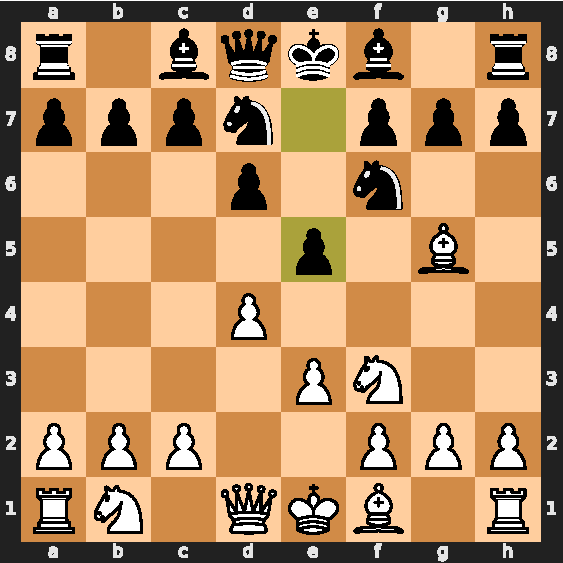
\includegraphics[width=108pt]{diagrams/board-f944b1b8af71}}};
\end{tikzpicture}

\vspace*{38pt}
\begin{center}
  \begin{minipage}{235pt}\centering
    {\fontsize{22}{25}\selectfont\bfseries Irregular Defence\par}
    \vspace{4pt}\rule{\linewidth}{1pt}\\[-9.5pt]\rule{\linewidth}{0.4pt}
  \end{minipage}

  \vspace{14pt}
  {\fontsize{19}{22}\selectfont\bfseries Janowski -- Capablanca\par}
  \vspace{10pt}
  {\fontsize{15}{18}\selectfont\bfseries Havana, 1913\par}
  \vspace{8pt}
  {\fontsize{11}{13}\selectfont White: D. Janowski \quad Black: J. R. Capablanca\par}
  \vspace{10pt}
  {\centering\fontsize{8.5}{10}\selectfont\itshape
   Notes by J. R. Capablanca, from \textup{Chess Fundamentals} (1921), which is in the public domain.\\
   Descriptive notation has been converted to algebraic. Page references are to the book.\\
   Click any move or diagram to open it on Lichess.\par}
\end{center}
\vspace{10pt}
}]
\textsizebook

\Move{\href{https://lichess.org/analysis/pgn/d4}{1.d4} \href{https://lichess.org/analysis/pgn/d4_Nf6}{\figN f6} \href{https://lichess.org/analysis/pgn/d4_Nf6_Nf3}{2.\figN f3} \href{https://lichess.org/analysis/pgn/d4_Nf6_Nf3_d6}{d6} \href{https://lichess.org/analysis/pgn/d4_Nf6_Nf3_d6_Bg5}{3.\figB g5} \href{https://lichess.org/analysis/pgn/d4_Nf6_Nf3_d6_Bg5_Nbd7}{\figN bd7} \href{https://lichess.org/analysis/pgn/d4_Nf6_Nf3_d6_Bg5_Nbd7_e3}{4.e3} \href{https://lichess.org/analysis/pgn/d4_Nf6_Nf3_d6_Bg5_Nbd7_e3_e5}{e5} \href{https://lichess.org/analysis/pgn/d4_Nf6_Nf3_d6_Bg5_Nbd7_e3_e5_Nc3}{5.\figN c3} \href{https://lichess.org/analysis/pgn/d4_Nf6_Nf3_d6_Bg5_Nbd7_e3_e5_Nc3_c6}{c6} \href{https://lichess.org/analysis/pgn/d4_Nf6_Nf3_d6_Bg5_Nbd7_e3_e5_Nc3_c6_Bd3}{6.\figB d3} \href{https://lichess.org/analysis/pgn/d4_Nf6_Nf3_d6_Bg5_Nbd7_e3_e5_Nc3_c6_Bd3_Be7}{\figB e7} \href{https://lichess.org/analysis/pgn/d4_Nf6_Nf3_d6_Bg5_Nbd7_e3_e5_Nc3_c6_Bd3_Be7_Qe2}{7.\figQ e2} \href{https://lichess.org/analysis/pgn/d4_Nf6_Nf3_d6_Bg5_Nbd7_e3_e5_Nc3_c6_Bd3_Be7_Qe2_Qa5}{\figQ a5} \href{https://lichess.org/analysis/pgn/d4_Nf6_Nf3_d6_Bg5_Nbd7_e3_e5_Nc3_c6_Bd3_Be7_Qe2_Qa5_O-O}{8.0--0} \href{https://lichess.org/analysis/pgn/d4_Nf6_Nf3_d6_Bg5_Nbd7_e3_e5_Nc3_c6_Bd3_Be7_Qe2_Qa5_O-O_Nf8}{\figN f8} \href{https://lichess.org/analysis/pgn/d4_Nf6_Nf3_d6_Bg5_Nbd7_e3_e5_Nc3_c6_Bd3_Be7_Qe2_Qa5_O-O_Nf8_Rfd1}{9.\figR fd1} \href{https://lichess.org/analysis/pgn/d4_Nf6_Nf3_d6_Bg5_Nbd7_e3_e5_Nc3_c6_Bd3_Be7_Qe2_Qa5_O-O_Nf8_Rfd1_Bg4}{\figB g4}}

At last Black is on his way to obtain full development. The idea of this irregular opening is mainly to throw White on his own resources. At the time the game was played, the system of defence was not as well known as the regular forms of the Queen's Pawn openings. Whether it is sound or not remains yet to be proved. Its good features are that it keeps the centre intact without creating any particular weakness, and that it gives plenty of opportunity for deep and concealed manoeuvring. The drawback is the long time it takes Black to develop his game. It is natural to suppose that White will employ that time to prepare a well-conceived attack, or that he will use the advantage of his development actually to prevent Black's complete development, or failing that, to obtain some definite material advantage.

\Move{\href{https://lichess.org/analysis/pgn/d4_Nf6_Nf3_d6_Bg5_Nbd7_e3_e5_Nc3_c6_Bd3_Be7_Qe2_Qa5_O-O_Nf8_Rfd1_Bg4_h3}{10.h3} \href{https://lichess.org/analysis/pgn/d4_Nf6_Nf3_d6_Bg5_Nbd7_e3_e5_Nc3_c6_Bd3_Be7_Qe2_Qa5_O-O_Nf8_Rfd1_Bg4_h3_Bh5}{\figB h5} \href{https://lichess.org/analysis/pgn/d4_Nf6_Nf3_d6_Bg5_Nbd7_e3_e5_Nc3_c6_Bd3_Be7_Qe2_Qa5_O-O_Nf8_Rfd1_Bg4_h3_Bh5_dxe5}{11.dxe5} \href{https://lichess.org/analysis/pgn/d4_Nf6_Nf3_d6_Bg5_Nbd7_e3_e5_Nc3_c6_Bd3_Be7_Qe2_Qa5_O-O_Nf8_Rfd1_Bg4_h3_Bh5_dxe5_dxe5}{dxe5} \href{https://lichess.org/analysis/pgn/d4_Nf6_Nf3_d6_Bg5_Nbd7_e3_e5_Nc3_c6_Bd3_Be7_Qe2_Qa5_O-O_Nf8_Rfd1_Bg4_h3_Bh5_dxe5_dxe5_Ne4}{12.\figN e4}}

\ChessDiagram{\href{https://lichess.org/analysis/pgn/d4_Nf6_Nf3_d6_Bg5_Nbd7_e3_e5_Nc3_c6_Bd3_Be7_Qe2_Qa5_O-O_Nf8_Rfd1_Bg4_h3_Bh5_dxe5_dxe5_Ne4}{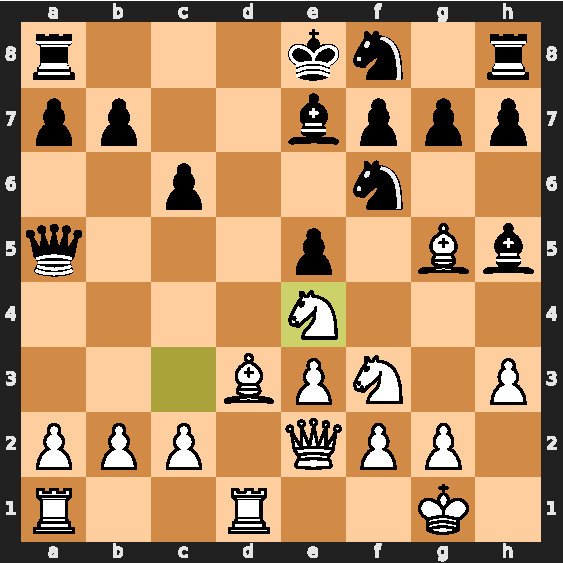
\includegraphics[width=\boardwidth]{diagrams/board-ace0c46345f0}}}

\Move{\href{https://lichess.org/analysis/pgn/d4_Nf6_Nf3_d6_Bg5_Nbd7_e3_e5_Nc3_c6_Bd3_Be7_Qe2_Qa5_O-O_Nf8_Rfd1_Bg4_h3_Bh5_dxe5_dxe5_Ne4_Nxe4}{12...\figN xe4}}

A very serious mistake. I considered castling (\href{https://lichess.org/analysis/pgn/d4_Nf6_Nf3_d6_Bg5_Nbd7_e3_e5_Nc3_c6_Bd3_Be7_Qe2_Qa5_O-O_Nf8_Rfd1_Bg4_h3_Bh5_dxe5_dxe5_Ne4_O-O-O}{12...0--0--0}), which was the right move, but desisted because I was afraid that by playing \href{https://lichess.org/analysis/pgn/d4_Nf6_Nf3_d6_Bg5_Nbd7_e3_e5_Nc3_c6_Bd3_Be7_Qe2_Qa5_O-O_Nf8_Rfd1_Bg4_h3_Bh5_dxe5_dxe5_Ne4_O-O-O_Bxf6}{13.\figB xf6} \href{https://lichess.org/analysis/pgn/d4_Nf6_Nf3_d6_Bg5_Nbd7_e3_e5_Nc3_c6_Bd3_Be7_Qe2_Qa5_O-O_Nf8_Rfd1_Bg4_h3_Bh5_dxe5_dxe5_Ne4_O-O-O_Bxf6_gxf6}{gxf6} \href{https://lichess.org/analysis/pgn/d4_Nf6_Nf3_d6_Bg5_Nbd7_e3_e5_Nc3_c6_Bd3_Be7_Qe2_Qa5_O-O_Nf8_Rfd1_Bg4_h3_Bh5_dxe5_dxe5_Ne4_O-O-O_Bxf6_gxf6_Ng3}{14.\figN g3} \href{https://lichess.org/analysis/pgn/d4_Nf6_Nf3_d6_Bg5_Nbd7_e3_e5_Nc3_c6_Bd3_Be7_Qe2_Qa5_O-O_Nf8_Rfd1_Bg4_h3_Bh5_dxe5_dxe5_Ne4_O-O-O_Bxf6_gxf6_Ng3_Bg6}{\figB g6} \href{https://lichess.org/analysis/pgn/d4_Nf6_Nf3_d6_Bg5_Nbd7_e3_e5_Nc3_c6_Bd3_Be7_Qe2_Qa5_O-O_Nf8_Rfd1_Bg4_h3_Bh5_dxe5_dxe5_Ne4_O-O-O_Bxf6_gxf6_Ng3_Bg6_Nf5}{15.\figN f5}, White would obtain a winning position for the end game. Whether right or wrong this shows how closely related are all parts of the game, and consequently how one will influence the other.

\Move{\href{https://lichess.org/analysis/pgn/d4_Nf6_Nf3_d6_Bg5_Nbd7_e3_e5_Nc3_c6_Bd3_Be7_Qe2_Qa5_O-O_Nf8_Rfd1_Bg4_h3_Bh5_dxe5_dxe5_Ne4_Nxe4_Bxe7}{13.\figB xe7} \href{https://lichess.org/analysis/pgn/d4_Nf6_Nf3_d6_Bg5_Nbd7_e3_e5_Nc3_c6_Bd3_Be7_Qe2_Qa5_O-O_Nf8_Rfd1_Bg4_h3_Bh5_dxe5_dxe5_Ne4_Nxe4_Bxe7_Kxe7}{\figK xe7} \href{https://lichess.org/analysis/pgn/d4_Nf6_Nf3_d6_Bg5_Nbd7_e3_e5_Nc3_c6_Bd3_Be7_Qe2_Qa5_O-O_Nf8_Rfd1_Bg4_h3_Bh5_dxe5_dxe5_Ne4_Nxe4_Bxe7_Kxe7_Bxe4}{14.\figB xe4} \href{https://lichess.org/analysis/pgn/d4_Nf6_Nf3_d6_Bg5_Nbd7_e3_e5_Nc3_c6_Bd3_Be7_Qe2_Qa5_O-O_Nf8_Rfd1_Bg4_h3_Bh5_dxe5_dxe5_Ne4_Nxe4_Bxe7_Kxe7_Bxe4_Bg6}{\figB g6}}

Not good. The natural and proper move would have been \href{https://lichess.org/analysis/pgn/d4_Nf6_Nf3_d6_Bg5_Nbd7_e3_e5_Nc3_c6_Bd3_Be7_Qe2_Qa5_O-O_Nf8_Rfd1_Bg4_h3_Bh5_dxe5_dxe5_Ne4_Nxe4_Bxe7_Kxe7_Bxe4_Ne6}{14...\figN e6}, in order to bring all the Black pieces into play. \href{https://lichess.org/analysis/pgn/d4_Nf6_Nf3_d6_Bg5_Nbd7_e3_e5_Nc3_c6_Bd3_Be7_Qe2_Qa5_O-O_Nf8_Rfd1_Bg4_h3_Bh5_dxe5_dxe5_Ne4_Nxe4_Bxe7_Kxe7_Bxe4_Bxf3}{14...\figB xf3} at once was also good, as it would have relieved the pressure against Black's King's Pawn, and at the same time have simplified the game.

Here it is seen how failure to comply with the elementary logical reasons, that govern any given position, often brings the player into trouble. I was no doubt influenced in my choice of moves by the fear of \figB f5, which was a very threatening move.

\Move{\href{https://lichess.org/analysis/pgn/d4_Nf6_Nf3_d6_Bg5_Nbd7_e3_e5_Nc3_c6_Bd3_Be7_Qe2_Qa5_O-O_Nf8_Rfd1_Bg4_h3_Bh5_dxe5_dxe5_Ne4_Nxe4_Bxe7_Kxe7_Bxe4_Bg6_Qc4}{15.\figQ c4} \href{https://lichess.org/analysis/pgn/d4_Nf6_Nf3_d6_Bg5_Nbd7_e3_e5_Nc3_c6_Bd3_Be7_Qe2_Qa5_O-O_Nf8_Rfd1_Bg4_h3_Bh5_dxe5_dxe5_Ne4_Nxe4_Bxe7_Kxe7_Bxe4_Bg6_Qc4_Ne6}{\figN e6} \href{https://lichess.org/analysis/pgn/d4_Nf6_Nf3_d6_Bg5_Nbd7_e3_e5_Nc3_c6_Bd3_Be7_Qe2_Qa5_O-O_Nf8_Rfd1_Bg4_h3_Bh5_dxe5_dxe5_Ne4_Nxe4_Bxe7_Kxe7_Bxe4_Bg6_Qc4_Ne6_b4}{16.b4} \href{https://lichess.org/analysis/pgn/d4_Nf6_Nf3_d6_Bg5_Nbd7_e3_e5_Nc3_c6_Bd3_Be7_Qe2_Qa5_O-O_Nf8_Rfd1_Bg4_h3_Bh5_dxe5_dxe5_Ne4_Nxe4_Bxe7_Kxe7_Bxe4_Bg6_Qc4_Ne6_b4_Qc7}{\figQ c7} \href{https://lichess.org/analysis/pgn/d4_Nf6_Nf3_d6_Bg5_Nbd7_e3_e5_Nc3_c6_Bd3_Be7_Qe2_Qa5_O-O_Nf8_Rfd1_Bg4_h3_Bh5_dxe5_dxe5_Ne4_Nxe4_Bxe7_Kxe7_Bxe4_Bg6_Qc4_Ne6_b4_Qc7_Bxg6}{17.\figB xg6} \href{https://lichess.org/analysis/pgn/d4_Nf6_Nf3_d6_Bg5_Nbd7_e3_e5_Nc3_c6_Bd3_Be7_Qe2_Qa5_O-O_Nf8_Rfd1_Bg4_h3_Bh5_dxe5_dxe5_Ne4_Nxe4_Bxe7_Kxe7_Bxe4_Bg6_Qc4_Ne6_b4_Qc7_Bxg6_hxg6}{hxg6} \href{https://lichess.org/analysis/pgn/d4_Nf6_Nf3_d6_Bg5_Nbd7_e3_e5_Nc3_c6_Bd3_Be7_Qe2_Qa5_O-O_Nf8_Rfd1_Bg4_h3_Bh5_dxe5_dxe5_Ne4_Nxe4_Bxe7_Kxe7_Bxe4_Bg6_Qc4_Ne6_b4_Qc7_Bxg6_hxg6_Qe4}{18.\figQ e4} \href{https://lichess.org/analysis/pgn/d4_Nf6_Nf3_d6_Bg5_Nbd7_e3_e5_Nc3_c6_Bd3_Be7_Qe2_Qa5_O-O_Nf8_Rfd1_Bg4_h3_Bh5_dxe5_dxe5_Ne4_Nxe4_Bxe7_Kxe7_Bxe4_Bg6_Qc4_Ne6_b4_Qc7_Bxg6_hxg6_Qe4_Kf6}{\figK f6}}

\ChessDiagram{\href{https://lichess.org/analysis/pgn/d4_Nf6_Nf3_d6_Bg5_Nbd7_e3_e5_Nc3_c6_Bd3_Be7_Qe2_Qa5_O-O_Nf8_Rfd1_Bg4_h3_Bh5_dxe5_dxe5_Ne4_Nxe4_Bxe7_Kxe7_Bxe4_Bg6_Qc4_Ne6_b4_Qc7_Bxg6_hxg6_Qe4_Kf6}{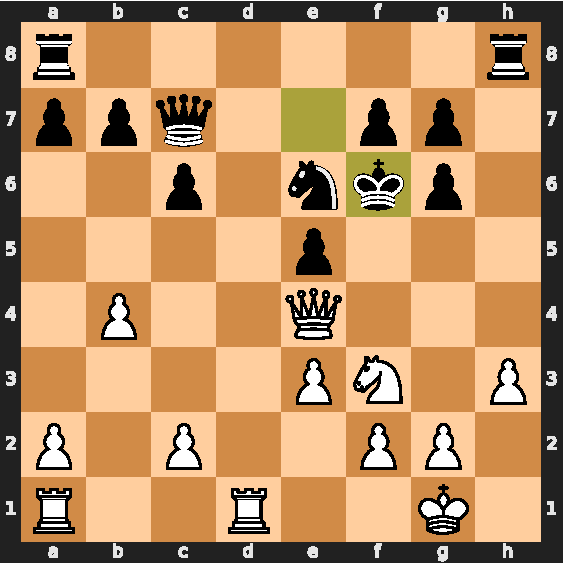
\includegraphics[width=\boardwidth]{diagrams/board-ae5cccbf73f6}}}

\Move{\href{https://lichess.org/analysis/pgn/d4_Nf6_Nf3_d6_Bg5_Nbd7_e3_e5_Nc3_c6_Bd3_Be7_Qe2_Qa5_O-O_Nf8_Rfd1_Bg4_h3_Bh5_dxe5_dxe5_Ne4_Nxe4_Bxe7_Kxe7_Bxe4_Bg6_Qc4_Ne6_b4_Qc7_Bxg6_hxg6_Qe4_Kf6_Rd3}{19.\figR d3}}

\href{https://lichess.org/analysis/pgn/d4_Nf6_Nf3_d6_Bg5_Nbd7_e3_e5_Nc3_c6_Bd3_Be7_Qe2_Qa5_O-O_Nf8_Rfd1_Bg4_h3_Bh5_dxe5_dxe5_Ne4_Nxe4_Bxe7_Kxe7_Bxe4_Bg6_Qc4_Ne6_b4_Qc7_Bxg6_hxg6_Qe4_Kf6_h4}{19.h4}, to be followed by g4, might have been a more vigorous way to carry on the attack. Black's weak point is unquestionably the Pawn at e5, which he is compelled to defend with the King. The text move aims at doubling the Rooks, with the ultimate object of placing one of them at d6, supported by a Pawn at c5, Black could only stop this by playing ...c5 which would create a ``hole'' at d5; or by playing ...b6, which would tie the Black Queen to the defence of the c-pawn as well as the e-pawn, which she already defends. Black, however, can meet all this by offering the exchange of Rooks, which destroys White's plans. For this reason \href{https://lichess.org/analysis/pgn/d4_Nf6_Nf3_d6_Bg5_Nbd7_e3_e5_Nc3_c6_Bd3_Be7_Qe2_Qa5_O-O_Nf8_Rfd1_Bg4_h3_Bh5_dxe5_dxe5_Ne4_Nxe4_Bxe7_Kxe7_Bxe4_Bg6_Qc4_Ne6_b4_Qc7_Bxg6_hxg6_Qe4_Kf6_h4}{19.h4} appears the proper way to carry on the attack.

\Move{\href{https://lichess.org/analysis/pgn/d4_Nf6_Nf3_d6_Bg5_Nbd7_e3_e5_Nc3_c6_Bd3_Be7_Qe2_Qa5_O-O_Nf8_Rfd1_Bg4_h3_Bh5_dxe5_dxe5_Ne4_Nxe4_Bxe7_Kxe7_Bxe4_Bg6_Qc4_Ne6_b4_Qc7_Bxg6_hxg6_Qe4_Kf6_Rd3_Rad8}{19...\figR ad8} \href{https://lichess.org/analysis/pgn/d4_Nf6_Nf3_d6_Bg5_Nbd7_e3_e5_Nc3_c6_Bd3_Be7_Qe2_Qa5_O-O_Nf8_Rfd1_Bg4_h3_Bh5_dxe5_dxe5_Ne4_Nxe4_Bxe7_Kxe7_Bxe4_Bg6_Qc4_Ne6_b4_Qc7_Bxg6_hxg6_Qe4_Kf6_Rd3_Rad8_Rad1}{20.\figR ad1} \href{https://lichess.org/analysis/pgn/d4_Nf6_Nf3_d6_Bg5_Nbd7_e3_e5_Nc3_c6_Bd3_Be7_Qe2_Qa5_O-O_Nf8_Rfd1_Bg4_h3_Bh5_dxe5_dxe5_Ne4_Nxe4_Bxe7_Kxe7_Bxe4_Bg6_Qc4_Ne6_b4_Qc7_Bxg6_hxg6_Qe4_Kf6_Rd3_Rad8_Rad1_g5}{g5}}

This move is preparatory to ...g6, which would make Black's position secure. Unfortunately for Black, he did not carry out his original plan.

\Move{\href{https://lichess.org/analysis/pgn/d4_Nf6_Nf3_d6_Bg5_Nbd7_e3_e5_Nc3_c6_Bd3_Be7_Qe2_Qa5_O-O_Nf8_Rfd1_Bg4_h3_Bh5_dxe5_dxe5_Ne4_Nxe4_Bxe7_Kxe7_Bxe4_Bg6_Qc4_Ne6_b4_Qc7_Bxg6_hxg6_Qe4_Kf6_Rd3_Rad8_Rad1_g5_c4}{21.c4} \href{https://lichess.org/analysis/pgn/d4_Nf6_Nf3_d6_Bg5_Nbd7_e3_e5_Nc3_c6_Bd3_Be7_Qe2_Qa5_O-O_Nf8_Rfd1_Bg4_h3_Bh5_dxe5_dxe5_Ne4_Nxe4_Bxe7_Kxe7_Bxe4_Bg6_Qc4_Ne6_b4_Qc7_Bxg6_hxg6_Qe4_Kf6_Rd3_Rad8_Rad1_g5_c4_Rxd3}{\figR xd3}}

\href{https://lichess.org/analysis/pgn/d4_Nf6_Nf3_d6_Bg5_Nbd7_e3_e5_Nc3_c6_Bd3_Be7_Qe2_Qa5_O-O_Nf8_Rfd1_Bg4_h3_Bh5_dxe5_dxe5_Ne4_Nxe4_Bxe7_Kxe7_Bxe4_Bg6_Qc4_Ne6_b4_Qc7_Bxg6_hxg6_Qe4_Kf6_Rd3_Rad8_Rad1_g5_c4_g6}{21...g6} would have left Black with a perfectly safe game.

\Move{\href{https://lichess.org/analysis/pgn/d4_Nf6_Nf3_d6_Bg5_Nbd7_e3_e5_Nc3_c6_Bd3_Be7_Qe2_Qa5_O-O_Nf8_Rfd1_Bg4_h3_Bh5_dxe5_dxe5_Ne4_Nxe4_Bxe7_Kxe7_Bxe4_Bg6_Qc4_Ne6_b4_Qc7_Bxg6_hxg6_Qe4_Kf6_Rd3_Rad8_Rad1_g5_c4_Rxd3_Rxd3}{22.\figR xd3} \href{https://lichess.org/analysis/pgn/d4_Nf6_Nf3_d6_Bg5_Nbd7_e3_e5_Nc3_c6_Bd3_Be7_Qe2_Qa5_O-O_Nf8_Rfd1_Bg4_h3_Bh5_dxe5_dxe5_Ne4_Nxe4_Bxe7_Kxe7_Bxe4_Bg6_Qc4_Ne6_b4_Qc7_Bxg6_hxg6_Qe4_Kf6_Rd3_Rad8_Rad1_g5_c4_Rxd3_Rxd3_Rd8}{\figR d8}}

A very serious mistake, which loses a Pawn. \href{https://lichess.org/analysis/pgn/d4_Nf6_Nf3_d6_Bg5_Nbd7_e3_e5_Nc3_c6_Bd3_Be7_Qe2_Qa5_O-O_Nf8_Rfd1_Bg4_h3_Bh5_dxe5_dxe5_Ne4_Nxe4_Bxe7_Kxe7_Bxe4_Bg6_Qc4_Ne6_b4_Qc7_Bxg6_hxg6_Qe4_Kf6_Rd3_Rad8_Rad1_g5_c4_Rxd3_Rxd3_g6}{22...g6} was the right move, and would have left Black with a very good game. In fact, if it should come to a simple ending, the position of the Black King would be an advantage.

\Move{\href{https://lichess.org/analysis/pgn/d4_Nf6_Nf3_d6_Bg5_Nbd7_e3_e5_Nc3_c6_Bd3_Be7_Qe2_Qa5_O-O_Nf8_Rfd1_Bg4_h3_Bh5_dxe5_dxe5_Ne4_Nxe4_Bxe7_Kxe7_Bxe4_Bg6_Qc4_Ne6_b4_Qc7_Bxg6_hxg6_Qe4_Kf6_Rd3_Rad8_Rad1_g5_c4_Rxd3_Rxd3_Rd8_Rxd8}{23.\figR xd8} \href{https://lichess.org/analysis/pgn/d4_Nf6_Nf3_d6_Bg5_Nbd7_e3_e5_Nc3_c6_Bd3_Be7_Qe2_Qa5_O-O_Nf8_Rfd1_Bg4_h3_Bh5_dxe5_dxe5_Ne4_Nxe4_Bxe7_Kxe7_Bxe4_Bg6_Qc4_Ne6_b4_Qc7_Bxg6_hxg6_Qe4_Kf6_Rd3_Rad8_Rad1_g5_c4_Rxd3_Rxd3_Rd8_Rxd8_Nxd8}{\figN xd8}}

\ChessDiagram{\href{https://lichess.org/analysis/pgn/d4_Nf6_Nf3_d6_Bg5_Nbd7_e3_e5_Nc3_c6_Bd3_Be7_Qe2_Qa5_O-O_Nf8_Rfd1_Bg4_h3_Bh5_dxe5_dxe5_Ne4_Nxe4_Bxe7_Kxe7_Bxe4_Bg6_Qc4_Ne6_b4_Qc7_Bxg6_hxg6_Qe4_Kf6_Rd3_Rad8_Rad1_g5_c4_Rxd3_Rxd3_Rd8_Rxd8_Nxd8}{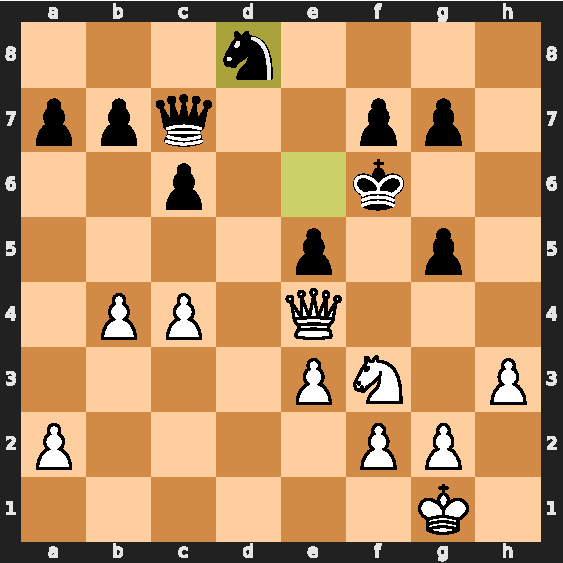
\includegraphics[width=\boardwidth]{diagrams/board-645ca91b5991}}}

\Move{\href{https://lichess.org/analysis/pgn/d4_Nf6_Nf3_d6_Bg5_Nbd7_e3_e5_Nc3_c6_Bd3_Be7_Qe2_Qa5_O-O_Nf8_Rfd1_Bg4_h3_Bh5_dxe5_dxe5_Ne4_Nxe4_Bxe7_Kxe7_Bxe4_Bg6_Qc4_Ne6_b4_Qc7_Bxg6_hxg6_Qe4_Kf6_Rd3_Rad8_Rad1_g5_c4_Rxd3_Rxd3_Rd8_Rxd8_Nxd8_h4}{24.h4}}

This wins a Pawn, as will soon be seen. Black cannot reply \href{https://lichess.org/analysis/pgn/d4_Nf6_Nf3_d6_Bg5_Nbd7_e3_e5_Nc3_c6_Bd3_Be7_Qe2_Qa5_O-O_Nf8_Rfd1_Bg4_h3_Bh5_dxe5_dxe5_Ne4_Nxe4_Bxe7_Kxe7_Bxe4_Bg6_Qc4_Ne6_b4_Qc7_Bxg6_hxg6_Qe4_Kf6_Rd3_Rad8_Rad1_g5_c4_Rxd3_Rxd3_Rd8_Rxd8_Nxd8_h4_Ne6}{24...\figN e6}; because \href{https://lichess.org/analysis/pgn/d4_Nf6_Nf3_d6_Bg5_Nbd7_e3_e5_Nc3_c6_Bd3_Be7_Qe2_Qa5_O-O_Nf8_Rfd1_Bg4_h3_Bh5_dxe5_dxe5_Ne4_Nxe4_Bxe7_Kxe7_Bxe4_Bg6_Qc4_Ne6_b4_Qc7_Bxg6_hxg6_Qe4_Kf6_Rd3_Rad8_Rad1_g5_c4_Rxd3_Rxd3_Rd8_Rxd8_Nxd8_h4_Ne6_hxg5}{25.hxg5+} \href{https://lichess.org/analysis/pgn/d4_Nf6_Nf3_d6_Bg5_Nbd7_e3_e5_Nc3_c6_Bd3_Be7_Qe2_Qa5_O-O_Nf8_Rfd1_Bg4_h3_Bh5_dxe5_dxe5_Ne4_Nxe4_Bxe7_Kxe7_Bxe4_Bg6_Qc4_Ne6_b4_Qc7_Bxg6_hxg6_Qe4_Kf6_Rd3_Rad8_Rad1_g5_c4_Rxd3_Rxd3_Rd8_Rxd8_Nxd8_h4_Ne6_hxg5_Nxg5}{\figN xg5} \href{https://lichess.org/analysis/pgn/d4_Nf6_Nf3_d6_Bg5_Nbd7_e3_e5_Nc3_c6_Bd3_Be7_Qe2_Qa5_O-O_Nf8_Rfd1_Bg4_h3_Bh5_dxe5_dxe5_Ne4_Nxe4_Bxe7_Kxe7_Bxe4_Bg6_Qc4_Ne6_b4_Qc7_Bxg6_hxg6_Qe4_Kf6_Rd3_Rad8_Rad1_g5_c4_Rxd3_Rxd3_Rd8_Rxd8_Nxd8_h4_Ne6_hxg5_Nxg5_Qh4}{26.\figQ h4} wins the Knight.

\Move{\href{https://lichess.org/analysis/pgn/d4_Nf6_Nf3_d6_Bg5_Nbd7_e3_e5_Nc3_c6_Bd3_Be7_Qe2_Qa5_O-O_Nf8_Rfd1_Bg4_h3_Bh5_dxe5_dxe5_Ne4_Nxe4_Bxe7_Kxe7_Bxe4_Bg6_Qc4_Ne6_b4_Qc7_Bxg6_hxg6_Qe4_Kf6_Rd3_Rad8_Rad1_g5_c4_Rxd3_Rxd3_Rd8_Rxd8_Nxd8_h4_gxh4}{24...gxh4} \href{https://lichess.org/analysis/pgn/d4_Nf6_Nf3_d6_Bg5_Nbd7_e3_e5_Nc3_c6_Bd3_Be7_Qe2_Qa5_O-O_Nf8_Rfd1_Bg4_h3_Bh5_dxe5_dxe5_Ne4_Nxe4_Bxe7_Kxe7_Bxe4_Bg6_Qc4_Ne6_b4_Qc7_Bxg6_hxg6_Qe4_Kf6_Rd3_Rad8_Rad1_g5_c4_Rxd3_Rxd3_Rd8_Rxd8_Nxd8_h4_gxh4_Qxh4}{25.\figQ xh4+} \href{https://lichess.org/analysis/pgn/d4_Nf6_Nf3_d6_Bg5_Nbd7_e3_e5_Nc3_c6_Bd3_Be7_Qe2_Qa5_O-O_Nf8_Rfd1_Bg4_h3_Bh5_dxe5_dxe5_Ne4_Nxe4_Bxe7_Kxe7_Bxe4_Bg6_Qc4_Ne6_b4_Qc7_Bxg6_hxg6_Qe4_Kf6_Rd3_Rad8_Rad1_g5_c4_Rxd3_Rxd3_Rd8_Rxd8_Nxd8_h4_gxh4_Qxh4_Ke6}{\figK e6} \href{https://lichess.org/analysis/pgn/d4_Nf6_Nf3_d6_Bg5_Nbd7_e3_e5_Nc3_c6_Bd3_Be7_Qe2_Qa5_O-O_Nf8_Rfd1_Bg4_h3_Bh5_dxe5_dxe5_Ne4_Nxe4_Bxe7_Kxe7_Bxe4_Bg6_Qc4_Ne6_b4_Qc7_Bxg6_hxg6_Qe4_Kf6_Rd3_Rad8_Rad1_g5_c4_Rxd3_Rxd3_Rd8_Rxd8_Nxd8_h4_gxh4_Qxh4_Ke6_Qg4}{26.\figQ g4+} \href{https://lichess.org/analysis/pgn/d4_Nf6_Nf3_d6_Bg5_Nbd7_e3_e5_Nc3_c6_Bd3_Be7_Qe2_Qa5_O-O_Nf8_Rfd1_Bg4_h3_Bh5_dxe5_dxe5_Ne4_Nxe4_Bxe7_Kxe7_Bxe4_Bg6_Qc4_Ne6_b4_Qc7_Bxg6_hxg6_Qe4_Kf6_Rd3_Rad8_Rad1_g5_c4_Rxd3_Rxd3_Rd8_Rxd8_Nxd8_h4_gxh4_Qxh4_Ke6_Qg4_Kf6}{\figK f6} \href{https://lichess.org/analysis/pgn/d4_Nf6_Nf3_d6_Bg5_Nbd7_e3_e5_Nc3_c6_Bd3_Be7_Qe2_Qa5_O-O_Nf8_Rfd1_Bg4_h3_Bh5_dxe5_dxe5_Ne4_Nxe4_Bxe7_Kxe7_Bxe4_Bg6_Qc4_Ne6_b4_Qc7_Bxg6_hxg6_Qe4_Kf6_Rd3_Rad8_Rad1_g5_c4_Rxd3_Rxd3_Rd8_Rxd8_Nxd8_h4_gxh4_Qxh4_Ke6_Qg4_Kf6_Qg5}{27.\figQ g5+} \href{https://lichess.org/analysis/pgn/d4_Nf6_Nf3_d6_Bg5_Nbd7_e3_e5_Nc3_c6_Bd3_Be7_Qe2_Qa5_O-O_Nf8_Rfd1_Bg4_h3_Bh5_dxe5_dxe5_Ne4_Nxe4_Bxe7_Kxe7_Bxe4_Bg6_Qc4_Ne6_b4_Qc7_Bxg6_hxg6_Qe4_Kf6_Rd3_Rad8_Rad1_g5_c4_Rxd3_Rxd3_Rd8_Rxd8_Nxd8_h4_gxh4_Qxh4_Ke6_Qg4_Kf6_Qg5_Ke6}{\figK e6} \href{https://lichess.org/analysis/pgn/d4_Nf6_Nf3_d6_Bg5_Nbd7_e3_e5_Nc3_c6_Bd3_Be7_Qe2_Qa5_O-O_Nf8_Rfd1_Bg4_h3_Bh5_dxe5_dxe5_Ne4_Nxe4_Bxe7_Kxe7_Bxe4_Bg6_Qc4_Ne6_b4_Qc7_Bxg6_hxg6_Qe4_Kf6_Rd3_Rad8_Rad1_g5_c4_Rxd3_Rxd3_Rd8_Rxd8_Nxd8_h4_gxh4_Qxh4_Ke6_Qg4_Kf6_Qg5_Ke6_Qxg7}{28.\figQ xg7} \href{https://lichess.org/analysis/pgn/d4_Nf6_Nf3_d6_Bg5_Nbd7_e3_e5_Nc3_c6_Bd3_Be7_Qe2_Qa5_O-O_Nf8_Rfd1_Bg4_h3_Bh5_dxe5_dxe5_Ne4_Nxe4_Bxe7_Kxe7_Bxe4_Bg6_Qc4_Ne6_b4_Qc7_Bxg6_hxg6_Qe4_Kf6_Rd3_Rad8_Rad1_g5_c4_Rxd3_Rxd3_Rd8_Rxd8_Nxd8_h4_gxh4_Qxh4_Ke6_Qg4_Kf6_Qg5_Ke6_Qxg7_Qd6}{\figQ d6} \href{https://lichess.org/analysis/pgn/d4_Nf6_Nf3_d6_Bg5_Nbd7_e3_e5_Nc3_c6_Bd3_Be7_Qe2_Qa5_O-O_Nf8_Rfd1_Bg4_h3_Bh5_dxe5_dxe5_Ne4_Nxe4_Bxe7_Kxe7_Bxe4_Bg6_Qc4_Ne6_b4_Qc7_Bxg6_hxg6_Qe4_Kf6_Rd3_Rad8_Rad1_g5_c4_Rxd3_Rxd3_Rd8_Rxd8_Nxd8_h4_gxh4_Qxh4_Ke6_Qg4_Kf6_Qg5_Ke6_Qxg7_Qd6_c5}{29.c5} \href{https://lichess.org/analysis/pgn/d4_Nf6_Nf3_d6_Bg5_Nbd7_e3_e5_Nc3_c6_Bd3_Be7_Qe2_Qa5_O-O_Nf8_Rfd1_Bg4_h3_Bh5_dxe5_dxe5_Ne4_Nxe4_Bxe7_Kxe7_Bxe4_Bg6_Qc4_Ne6_b4_Qc7_Bxg6_hxg6_Qe4_Kf6_Rd3_Rad8_Rad1_g5_c4_Rxd3_Rxd3_Rd8_Rxd8_Nxd8_h4_gxh4_Qxh4_Ke6_Qg4_Kf6_Qg5_Ke6_Qxg7_Qd6_c5_Qd5}{\figQ d5} \href{https://lichess.org/analysis/pgn/d4_Nf6_Nf3_d6_Bg5_Nbd7_e3_e5_Nc3_c6_Bd3_Be7_Qe2_Qa5_O-O_Nf8_Rfd1_Bg4_h3_Bh5_dxe5_dxe5_Ne4_Nxe4_Bxe7_Kxe7_Bxe4_Bg6_Qc4_Ne6_b4_Qc7_Bxg6_hxg6_Qe4_Kf6_Rd3_Rad8_Rad1_g5_c4_Rxd3_Rxd3_Rd8_Rxd8_Nxd8_h4_gxh4_Qxh4_Ke6_Qg4_Kf6_Qg5_Ke6_Qxg7_Qd6_c5_Qd5_e4}{30.e4!} \href{https://lichess.org/analysis/pgn/d4_Nf6_Nf3_d6_Bg5_Nbd7_e3_e5_Nc3_c6_Bd3_Be7_Qe2_Qa5_O-O_Nf8_Rfd1_Bg4_h3_Bh5_dxe5_dxe5_Ne4_Nxe4_Bxe7_Kxe7_Bxe4_Bg6_Qc4_Ne6_b4_Qc7_Bxg6_hxg6_Qe4_Kf6_Rd3_Rad8_Rad1_g5_c4_Rxd3_Rxd3_Rd8_Rxd8_Nxd8_h4_gxh4_Qxh4_Ke6_Qg4_Kf6_Qg5_Ke6_Qxg7_Qd6_c5_Qd5_e4_Qd1}{\figQ d1+} \href{https://lichess.org/analysis/pgn/d4_Nf6_Nf3_d6_Bg5_Nbd7_e3_e5_Nc3_c6_Bd3_Be7_Qe2_Qa5_O-O_Nf8_Rfd1_Bg4_h3_Bh5_dxe5_dxe5_Ne4_Nxe4_Bxe7_Kxe7_Bxe4_Bg6_Qc4_Ne6_b4_Qc7_Bxg6_hxg6_Qe4_Kf6_Rd3_Rad8_Rad1_g5_c4_Rxd3_Rxd3_Rd8_Rxd8_Nxd8_h4_gxh4_Qxh4_Ke6_Qg4_Kf6_Qg5_Ke6_Qxg7_Qd6_c5_Qd5_e4_Qd1_Kh2}{31.\figK h2} \href{https://lichess.org/analysis/pgn/d4_Nf6_Nf3_d6_Bg5_Nbd7_e3_e5_Nc3_c6_Bd3_Be7_Qe2_Qa5_O-O_Nf8_Rfd1_Bg4_h3_Bh5_dxe5_dxe5_Ne4_Nxe4_Bxe7_Kxe7_Bxe4_Bg6_Qc4_Ne6_b4_Qc7_Bxg6_hxg6_Qe4_Kf6_Rd3_Rad8_Rad1_g5_c4_Rxd3_Rxd3_Rd8_Rxd8_Nxd8_h4_gxh4_Qxh4_Ke6_Qg4_Kf6_Qg5_Ke6_Qxg7_Qd6_c5_Qd5_e4_Qd1_Kh2_f6}{f6} \href{https://lichess.org/analysis/pgn/d4_Nf6_Nf3_d6_Bg5_Nbd7_e3_e5_Nc3_c6_Bd3_Be7_Qe2_Qa5_O-O_Nf8_Rfd1_Bg4_h3_Bh5_dxe5_dxe5_Ne4_Nxe4_Bxe7_Kxe7_Bxe4_Bg6_Qc4_Ne6_b4_Qc7_Bxg6_hxg6_Qe4_Kf6_Rd3_Rad8_Rad1_g5_c4_Rxd3_Rxd3_Rd8_Rxd8_Nxd8_h4_gxh4_Qxh4_Ke6_Qg4_Kf6_Qg5_Ke6_Qxg7_Qd6_c5_Qd5_e4_Qd1_Kh2_f6_Qg4}{32.\figQ g4+!} \href{https://lichess.org/analysis/pgn/d4_Nf6_Nf3_d6_Bg5_Nbd7_e3_e5_Nc3_c6_Bd3_Be7_Qe2_Qa5_O-O_Nf8_Rfd1_Bg4_h3_Bh5_dxe5_dxe5_Ne4_Nxe4_Bxe7_Kxe7_Bxe4_Bg6_Qc4_Ne6_b4_Qc7_Bxg6_hxg6_Qe4_Kf6_Rd3_Rad8_Rad1_g5_c4_Rxd3_Rxd3_Rd8_Rxd8_Nxd8_h4_gxh4_Qxh4_Ke6_Qg4_Kf6_Qg5_Ke6_Qxg7_Qd6_c5_Qd5_e4_Qd1_Kh2_f6_Qg4_Ke7}{\figK e7} \href{https://lichess.org/analysis/pgn/d4_Nf6_Nf3_d6_Bg5_Nbd7_e3_e5_Nc3_c6_Bd3_Be7_Qe2_Qa5_O-O_Nf8_Rfd1_Bg4_h3_Bh5_dxe5_dxe5_Ne4_Nxe4_Bxe7_Kxe7_Bxe4_Bg6_Qc4_Ne6_b4_Qc7_Bxg6_hxg6_Qe4_Kf6_Rd3_Rad8_Rad1_g5_c4_Rxd3_Rxd3_Rd8_Rxd8_Nxd8_h4_gxh4_Qxh4_Ke6_Qg4_Kf6_Qg5_Ke6_Qxg7_Qd6_c5_Qd5_e4_Qd1_Kh2_f6_Qg4_Ke7_Nxe5}{33.\figN xe5} \href{https://lichess.org/analysis/pgn/d4_Nf6_Nf3_d6_Bg5_Nbd7_e3_e5_Nc3_c6_Bd3_Be7_Qe2_Qa5_O-O_Nf8_Rfd1_Bg4_h3_Bh5_dxe5_dxe5_Ne4_Nxe4_Bxe7_Kxe7_Bxe4_Bg6_Qc4_Ne6_b4_Qc7_Bxg6_hxg6_Qe4_Kf6_Rd3_Rad8_Rad1_g5_c4_Rxd3_Rxd3_Rd8_Rxd8_Nxd8_h4_gxh4_Qxh4_Ke6_Qg4_Kf6_Qg5_Ke6_Qxg7_Qd6_c5_Qd5_e4_Qd1_Kh2_f6_Qg4_Ke7_Nxe5_Qxg4}{\figQ xg4} \href{https://lichess.org/analysis/pgn/d4_Nf6_Nf3_d6_Bg5_Nbd7_e3_e5_Nc3_c6_Bd3_Be7_Qe2_Qa5_O-O_Nf8_Rfd1_Bg4_h3_Bh5_dxe5_dxe5_Ne4_Nxe4_Bxe7_Kxe7_Bxe4_Bg6_Qc4_Ne6_b4_Qc7_Bxg6_hxg6_Qe4_Kf6_Rd3_Rad8_Rad1_g5_c4_Rxd3_Rxd3_Rd8_Rxd8_Nxd8_h4_gxh4_Qxh4_Ke6_Qg4_Kf6_Qg5_Ke6_Qxg7_Qd6_c5_Qd5_e4_Qd1_Kh2_f6_Qg4_Ke7_Nxe5_Qxg4_Nxg4}{34.\figN xg4} \href{https://lichess.org/analysis/pgn/d4_Nf6_Nf3_d6_Bg5_Nbd7_e3_e5_Nc3_c6_Bd3_Be7_Qe2_Qa5_O-O_Nf8_Rfd1_Bg4_h3_Bh5_dxe5_dxe5_Ne4_Nxe4_Bxe7_Kxe7_Bxe4_Bg6_Qc4_Ne6_b4_Qc7_Bxg6_hxg6_Qe4_Kf6_Rd3_Rad8_Rad1_g5_c4_Rxd3_Rxd3_Rd8_Rxd8_Nxd8_h4_gxh4_Qxh4_Ke6_Qg4_Kf6_Qg5_Ke6_Qxg7_Qd6_c5_Qd5_e4_Qd1_Kh2_f6_Qg4_Ke7_Nxe5_Qxg4_Nxg4_Ne6}{\figN e6} \href{https://lichess.org/analysis/pgn/d4_Nf6_Nf3_d6_Bg5_Nbd7_e3_e5_Nc3_c6_Bd3_Be7_Qe2_Qa5_O-O_Nf8_Rfd1_Bg4_h3_Bh5_dxe5_dxe5_Ne4_Nxe4_Bxe7_Kxe7_Bxe4_Bg6_Qc4_Ne6_b4_Qc7_Bxg6_hxg6_Qe4_Kf6_Rd3_Rad8_Rad1_g5_c4_Rxd3_Rxd3_Rd8_Rxd8_Nxd8_h4_gxh4_Qxh4_Ke6_Qg4_Kf6_Qg5_Ke6_Qxg7_Qd6_c5_Qd5_e4_Qd1_Kh2_f6_Qg4_Ke7_Nxe5_Qxg4_Nxg4_Ne6_e5}{35.e5} \href{https://lichess.org/analysis/pgn/d4_Nf6_Nf3_d6_Bg5_Nbd7_e3_e5_Nc3_c6_Bd3_Be7_Qe2_Qa5_O-O_Nf8_Rfd1_Bg4_h3_Bh5_dxe5_dxe5_Ne4_Nxe4_Bxe7_Kxe7_Bxe4_Bg6_Qc4_Ne6_b4_Qc7_Bxg6_hxg6_Qe4_Kf6_Rd3_Rad8_Rad1_g5_c4_Rxd3_Rxd3_Rd8_Rxd8_Nxd8_h4_gxh4_Qxh4_Ke6_Qg4_Kf6_Qg5_Ke6_Qxg7_Qd6_c5_Qd5_e4_Qd1_Kh2_f6_Qg4_Ke7_Nxe5_Qxg4_Nxg4_Ne6_e5_fxe5}{fxe5} \href{https://lichess.org/analysis/pgn/d4_Nf6_Nf3_d6_Bg5_Nbd7_e3_e5_Nc3_c6_Bd3_Be7_Qe2_Qa5_O-O_Nf8_Rfd1_Bg4_h3_Bh5_dxe5_dxe5_Ne4_Nxe4_Bxe7_Kxe7_Bxe4_Bg6_Qc4_Ne6_b4_Qc7_Bxg6_hxg6_Qe4_Kf6_Rd3_Rad8_Rad1_g5_c4_Rxd3_Rxd3_Rd8_Rxd8_Nxd8_h4_gxh4_Qxh4_Ke6_Qg4_Kf6_Qg5_Ke6_Qxg7_Qd6_c5_Qd5_e4_Qd1_Kh2_f6_Qg4_Ke7_Nxe5_Qxg4_Nxg4_Ne6_e5_fxe5_Nxe5}{36.\figN xe5} \href{https://lichess.org/analysis/pgn/d4_Nf6_Nf3_d6_Bg5_Nbd7_e3_e5_Nc3_c6_Bd3_Be7_Qe2_Qa5_O-O_Nf8_Rfd1_Bg4_h3_Bh5_dxe5_dxe5_Ne4_Nxe4_Bxe7_Kxe7_Bxe4_Bg6_Qc4_Ne6_b4_Qc7_Bxg6_hxg6_Qe4_Kf6_Rd3_Rad8_Rad1_g5_c4_Rxd3_Rxd3_Rd8_Rxd8_Nxd8_h4_gxh4_Qxh4_Ke6_Qg4_Kf6_Qg5_Ke6_Qxg7_Qd6_c5_Qd5_e4_Qd1_Kh2_f6_Qg4_Ke7_Nxe5_Qxg4_Nxg4_Ne6_e5_fxe5_Nxe5_Nd4}{\figN d4}}

The game went on for a few more moves, and, there being no way to counteract the advance of White's two passed Pawns, Black resigned.

\end{document}
